\documentclass[aspectratio=169, 10pt]{beamer}
\usepackage[utf8]{inputenc}
\usepackage{amsmath, amssymb, bm, amsfonts}
\usepackage{booktabs}
\usepackage{listings}
\usepackage{graphicx}
\usepackage{tikz}
\usetikzlibrary{arrows.meta, positioning, calc, angles, quotes, shapes.geometric, decorations.pathmorphing}

% ==============================================================================
% THEME & UNIVERSIDAD DE ANTIOQUIA (UdeA) BRANDING SETUP
% ==============================================================================
\usetheme{Madrid}
\usefonttheme{professionalfonts}

\definecolor{UdeAGreen}{HTML}{006241}
\definecolor{UdeAGold}{HTML}{D4AF37}
\definecolor{Charcoal}{HTML}{2B2B2B}
\definecolor{LightBg}{HTML}{F8F9FA}
\definecolor{DarkSlate}{RGB}{15, 23, 42}
\definecolor{AlertRed}{RGB}{220, 38, 38}
\definecolor{SpiceBlue}{RGB}{2, 132, 199}

\setbeamercolor{palette primary}{bg=UdeAGreen, fg=white}
\setbeamercolor{palette secondary}{bg=UdeAGreen, fg=white}
\setbeamercolor{palette tertiary}{bg=UdeAGreen, fg=white}
\setbeamercolor{structure}{fg=UdeAGreen}
\setbeamercolor{background canvas}{bg=LightBg}
\setbeamercolor{text}{fg=Charcoal}

% Infolines Header/Footline Colors
\setbeamercolor{author in head/foot}{bg=UdeAGreen, fg=white}
\setbeamercolor{title in head/foot}{bg=UdeAGreen, fg=white}
\setbeamercolor{date in head/foot}{bg=UdeAGreen, fg=white}

% Block Styles
\setbeamercolor{block title}{bg=UdeAGreen, fg=white}
\setbeamercolor{block body}{bg=white, fg=Charcoal}
\setbeamercolor{block title example}{bg=UdeAGold, fg=DarkSlate}
\setbeamercolor{block body example}{bg=white, fg=Charcoal}
\setbeamercolor{block title alerted}{bg=AlertRed, fg=white}
\setbeamercolor{block body alerted}{bg=white, fg=Charcoal}

% Header & Footer Setup Matching Module 3
\setbeamertemplate{headline}{}
\setbeamertemplate{navigation symbols}{}

\setbeamertemplate{footline}{%
    \leavevmode%
    \hbox{%
        \begin{beamercolorbox}[wd=.333333\paperwidth,ht=2.25ex,dp=1ex,center]{author in head/foot}%
            \usebeamerfont{author in head/foot}\insertshortauthor~~(\insertshortinstitute)%
        \end{beamercolorbox}%
        \begin{beamercolorbox}[wd=.333333\paperwidth,ht=2.25ex,dp=1ex,center]{title in head/foot}%
            \usebeamerfont{title in head/foot}\insertshorttitle
        \end{beamercolorbox}%
        \begin{beamercolorbox}[wd=.333333\paperwidth,ht=2.25ex,dp=1ex,right]{date in head/foot}%
            \usebeamerfont{date in head/foot}\insertshortdate{}\hspace*{2em}
            \insertframenumber{} / \inserttotalframenumber\hspace*{2ex} 
        \end{beamercolorbox}%
    }%
    \vskip0pt%
}

% Logo positioned above the footer in the bottom right corner
\logo{%
    \vspace{-0.2cm}\hfill%
    \IfFileExists{Images/UdeA+simplificado+Negro_Smaller.png}{%
        
\includegraphics[width=1cm]{Images/UdeA+simplificado+Negro_Smaller.png}%
    }{%
        \textbf{UdeA}%
    }%
    \hspace{0.1cm}%
}

% Code Listings Configuration
\lstdefinestyle{gmatstyle}{
    backgroundcolor=\color{LightBg},
    basicstyle=\ttfamily\fontsize{5pt}{6pt}\selectfont\color{Charcoal},
    keywordstyle=\bfseries\color{UdeAGreen},
    commentstyle=\itshape\color{gray},
    stringstyle=\color{UdeAGold!90!black},
    frame=single,
    rulecolor=\color{UdeAGreen},
    breaklines=true,
    showstringspaces=false,
    xleftmargin=3pt,
    xrightmargin=3pt
}

\lstdefinestyle{pythoncode}{
    backgroundcolor=\color{white},
    basicstyle=\ttfamily\fontsize{5.0pt}{6.0pt}\selectfont\color{Charcoal},
    keywordstyle=\bfseries\color{UdeAGreen},
    commentstyle=\itshape\color{gray},
    stringstyle=\color{UdeAGold!90!black},
    numberstyle=\tiny\color{gray},
    numbers=left,
    numbersep=3pt,
    frame=single,
    rulecolor=\color{UdeAGreen!50},
    breaklines=true,
    showstringspaces=false,
    tabsize=2,
    xleftmargin=3pt,
    xrightmargin=3pt
}

% Presentation Metadata with short forms for the three-block footline
\title[Astrodynamics Module 4]{\textbf{Module 4: Multi-Body Dynamics and Symplectic Sandbox}}
\subtitle{The Circular Restricted Three-Body Problem (CR3BP) and Cislunar Mission Design}
\author[Juan Francisco Puerta Ibarra]{\textbf{Juan Francisco Puerta Ibarra}}
\institute[Aerospace Engineering]{Department of Aerospace Engineering --- Faculty of Engineering \\ Universidad de Antioquia (UdeA)}
\date[Semester 2026-2]{Semester 2026-2}
\titlegraphic{%
    \IfFileExists{Images/UdeA+simplificado+Negro_Smaller.png}{%
        
\includegraphics[width=2.5cm,keepaspectratio]{Images/UdeA+simplificado+Negro_Smaller.png}%
    }{}%
}

\begin{document}

% ==============================================================================
% SLIDE 1: TITLE SLIDE
% ==============================================================================
\begin{frame}[plain]
    \titlepage
    \begin{center}
        \scriptsize \textcolor{DarkSlate}{\textit{Analytical Flight Mechanics, Invariant Manifold Theory, and Symplectic Sandbox Propagation}}
    \end{center}
\end{frame}

% ==============================================================================
% SLIDE 2: MODULE ROADMAP
% ==============================================================================
\begin{frame}{Module 4 Curriculum Roadmap: Multi-Body Astrodynamics}
    \begin{columns}[t]
        \begin{column}{0.32\textwidth}
            \begin{block}{\textbf{Week 11: The Synodic Frame}}
                \scriptsize
                \begin{itemize}\setlength{\itemsep}{3pt}
                    \item \textbf{Breakdown of 2-Body}: Gravitational competition in cislunar space.
                    \item \textbf{Rotating Coordinates}: Transport theorem, barycentric axes.
                    \item \textbf{CR3BP Equations}: Canonical normalization ($\mu$).
                    \item \textbf{Jacobi Constant ($C$)}: First integral and conservation metric.
                    \item \textbf{Zero-Velocity Surfaces}: Hill regions and energy gateways.
                \end{itemize}
            \end{block}
        \end{column}
        
        \begin{column}{0.32\textwidth}
            \begin{block}{\textbf{Week 12: Libration Dynamics}}
                \scriptsize
                \begin{itemize}\setlength{\itemsep}{3pt}
                    \item \textbf{Equilibrium Points}: Collinear ($L_1, L_2, L_3$) and Triangular ($L_4, L_5$).
                    \item \textbf{Linearization}: Eigenstructure of the variational matrix.
                    \item \textbf{Periodic Orbits}: Planar Lyapunov, vertical, and 3D Halo orbits.
                    \item \textbf{Richardson Expansions}: 3rd-order analytical seed generation.
                    \item \textbf{Computational Lab 3}: Non-symplectic vs. Symplectic integrators.
                \end{itemize}
            \end{block}
        \end{column}
        
        \begin{column}{0.32\textwidth}
            \begin{block}{\textbf{Week 13: Cislunar Transit}}
                \scriptsize
                \begin{itemize}\setlength{\itemsep}{3pt}
                    \item \textbf{Monodromy Matrix}: Floquet multipliers and orbital stability.
                    \item \textbf{Invariant Manifolds}: Stable ($W^s$) and unstable ($W^u$) tube structures.
                    \item \textbf{Heteroclinic Bridges}: Low-energy orbital connections.
                    \item \textbf{Mission Architecture}: Lunar Gateway NRHO, GRAIL ballistic capture.
                    \item \textbf{NASA GMAT}: Full ephemeris operational transition.
                \end{itemize}
            \end{block}
        \end{column}
    \end{columns}
\end{frame}

% ==============================================================================
% SLIDE 3: BEYOND THE KEPLERIAN TWO-BODY PROBLEM
% ==============================================================================
\begin{frame}{The Breakdown of Keplerian Mechanics in Cislunar Space}
    \begin{columns}[t]
        \begin{column}{0.49\textwidth}
            \begin{block}{\textbf{The Classical 2-Body Limitation}}
                \scriptsize
                In two-body mechanics (R2BP), motion is completely integrable:
                \begin{itemize}\setlength{\itemsep}{1.5pt}
                    \item Closed-form conic trajectories (ellipses, hyperbolas).
                    \item Mechanical energy $\mathcal{E}$ and angular momentum $\mathbf{h}$ are strictly conserved vectors.
                    \item Patched Conics assumes instantaneous spheres of influence (SOI).
                \end{itemize}
            \end{block}
            \vspace{-0.15cm}
            \begin{alertblock}{\textbf{The Cislunar Reality}}
                \scriptsize
                Between Earth and Moon, both gravitational fields act continuously:
                \begin{itemize}\setlength{\itemsep}{1.5pt}
                    \item No general analytical solution exists (Poincaré non-integrability).
                    \item $\mathcal{E}$ and $\mathbf{h}$ fluctuate rapidly; orbits are non-Keplerian.
                \end{itemize}
            \end{alertblock}
        \end{column}
        
        \begin{column}{0.48\textwidth}
            \begin{exampleblock}{\textbf{Comparative Dynamics Framework}}
                \scriptsize
                \centering
                \resizebox{\linewidth}{!}{%
                \begin{tabular}{lcc}
                    \toprule
                    \textbf{Property} & \textbf{Kepler (2-Body)} & \textbf{CR3BP} \\
                    \midrule
                    Integrals of Motion & 10 classical & 1 Jacobi Constant ($C$) \\
                    Trajectories & Pure conics & Chaotic / Resonant \\
                    Equilibria & Central attractor & 5 Libration points \\
                    Transfers & High-$\Delta V$ Hohmann & Low-energy tube transits \\
                    Frame of Reference & Inertial ECI & Synodic (Rotating) \\
                    \bottomrule
                \end{tabular}%
                }
            \end{exampleblock}
            \vspace{0.05cm}
            \begin{center}
                \scriptsize \textcolor{DarkSlate}{\textit{"In multi-body regimes, gravitational fields do not compete; they cooperate to form dynamical transport highways."}}
            \end{center}
        \end{column}
    \end{columns}
\end{frame}

% ==============================================================================
% SLIDE 4: THE CIRCULAR RESTRICTED THREE-BODY PROBLEM (CR3BP)
% ==============================================================================
\begin{frame}{Formulation of the CR3BP}
    \begin{columns}[t]
        \begin{column}{0.52\textwidth}
            \begin{block}{\textbf{Fundamental Model Assumptions}}
                \scriptsize
                The Circular Restricted Three-Body Problem models third-body flight under physically grounded simplifications:
                \begin{enumerate}\setlength{\itemsep}{2pt}
                    \item \textbf{Primaries ($m_1, m_2$):} Move in circular coplanar orbits about their mutual barycenter at constant angular velocity $\Omega$.
                    \item \textbf{Third Body ($m$):} Negligible mass ($m \ll m_1, m_2$). Influenced by both primaries but exerts \textbf{no back-reaction}.
                    \item \textbf{Isolated System:} Neglect solar tides, planetary oblateness ($J_2$), and non-gravitational perturbations in canonical form.
                \end{enumerate}
            \end{block}
        \end{column}
        
        \begin{column}{0.45\textwidth}
            \begin{block}{\textbf{Canonical Non-Dimensional Units}}
                \scriptsize
                Define characteristic scales to set physical constants to unity:
                \begin{align*}
                    [L] &= R = r_1 + r_2 = 1 \\
                    [M] &= m_1 + m_2 = 1, \quad [T] = \frac{1}{\Omega} = 1
                \end{align*}
                Consequences of canonical scaling:
                \begin{itemize}\setlength{\itemsep}{2pt}
                    \item Gravitational constant: $G = 1$.
                    \item Mean motion: $\Omega = \sqrt{G(m_1 + m_2)/R^3} = 1$.
                    \item Orbital period of primaries: $T = 2\pi$.
                    \item \textbf{Mass Parameter ($\mu$):}
                    \begin{equation*}
                        \mu = \frac{m_2}{m_1 + m_2} \implies m_1 = 1 - \mu, \quad m_2 = \mu
                    \end{equation*}
                \end{itemize}
            \end{block}
        \end{column}
    \end{columns}
\end{frame}

% ==============================================================================
% SLIDE 5: KINEMATICS IN THE SYNODIC FRAME
% ==============================================================================
\begin{frame}{Kinematics in the Synodic (Rotating) Reference Frame}
    \begin{columns}[t]
        \begin{column}{0.50\textwidth}
            \begin{block}{\textbf{Transport Theorem Acceleration}}
                \scriptsize
                Let $\mathcal{I}$ be the inertial barycentric frame and $\mathcal{R}$ the frame corotating at $\bm{\omega} = \Omega \hat{\mathbf{z}} = 1\hat{\mathbf{z}}$:
                \begin{equation*}
                    \left(\frac{d\mathbf{r}}{dt}\right)_\mathcal{I} = \left(\frac{d\mathbf{r}}{dt}\right)_\mathcal{R} + \bm{\omega} \times \mathbf{r} = \mathbf{v}_\mathcal{R} + \bm{\omega} \times \mathbf{r}
                \end{equation*}
                Differentiating again yields total inertial acceleration:
                \begin{equation*}
                    \mathbf{a}_\mathcal{I} = \ddot{\mathbf{r}}_\mathcal{R} + 2\bm{\omega} \times \dot{\mathbf{r}}_\mathcal{R} + \bm{\omega} \times (\bm{\omega} \times \mathbf{r})
                \end{equation*}
                The apparent kinematic accelerations are:
                \begin{itemize}\setlength{\itemsep}{1.5pt}
                    \item $\mathbf{a}_{\text{cor}} = 2\bm{\omega} \times \dot{\mathbf{r}}_\mathcal{R} = [-2\dot{y}, 2\dot{x}, 0]^T$ (Coriolis).
                    \item $\mathbf{a}_{\text{cen}} = \bm{\omega} \times (\bm{\omega} \times \mathbf{r}) = [-x, -y, 0]^T$ (Centrifugal).
                \end{itemize}
            \end{block}
        \end{column}
        
        \begin{column}{0.47\textwidth}
            \begin{block}{\textbf{Geometric State Coordinates}}
                \scriptsize
                The primaries are pinned along the synodic $x$-axis:
                \begin{itemize}\setlength{\itemsep}{1.5pt}
                    \item Primary $m_1$ (Earth): $\mathbf{r}_{m1} = [-\mu, 0, 0]^T$
                    \item Secondary $m_2$ (Moon): $\mathbf{r}_{m2} = [1-\mu, 0, 0]^T$
                    \item Spacecraft $P$: $\mathbf{r} = [x, y, z]^T$
                \end{itemize}
                Relative distance scalar norms:
                \begin{align*}
                    d_1 &= \sqrt{(x + \mu)^2 + y^2 + z^2} \\
                    d_2 &= \sqrt{(x - 1 + \mu)^2 + y^2 + z^2}
                \end{align*}
                \vspace{-0.3cm}
                Newton's second law in rotating form:
                {\scriptsize
                \begin{equation*}
                    \ddot{\mathbf{r}}_\mathcal{R} + 2\bm{\omega} \times \dot{\mathbf{r}}_\mathcal{R} + \bm{\omega} \times (\bm{\omega} \times \mathbf{r}) = -\frac{1-\mu}{d_1^3}\mathbf{d}_1 - \frac{\mu}{d_2^3}\mathbf{d}_2
                \end{equation*}}
            \end{block}
        \end{column}
    \end{columns}
\end{frame}

% ==============================================================================
% SLIDE 6: SYNODIC FRAME GEOMETRY (TIKZ DIAGRAM)
% ==============================================================================
\begin{frame}{Synodic Reference Frame Geometry}
    \begin{center}
        \vspace{-0.15cm}
        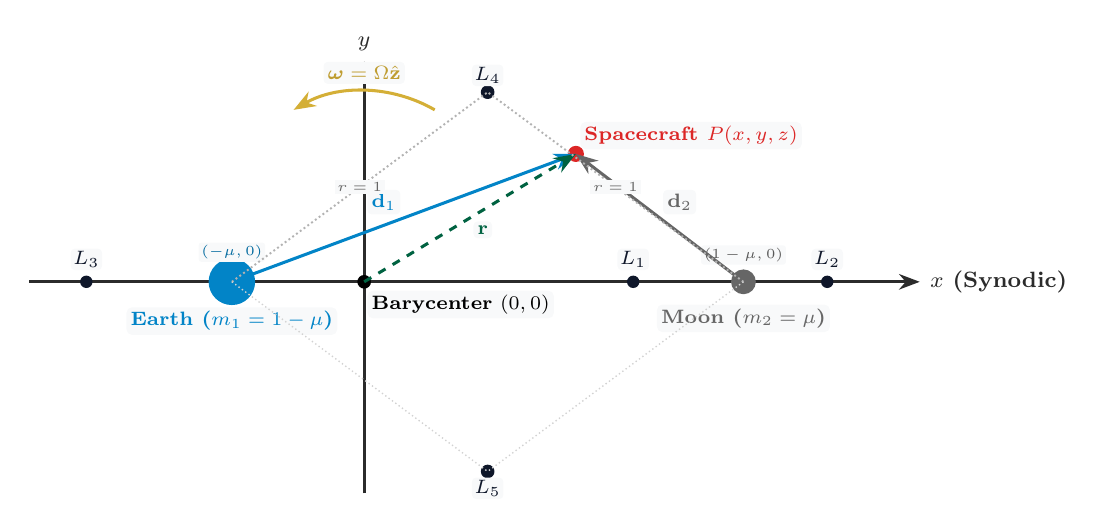
\begin{tikzpicture}[scale=1.12, >=Stealth]
            % Barycenter Origin
            \coordinate (B) at (0,0);
            
            % Coordinate Axes
            \draw[->, line width=1.0pt, Charcoal] (-3.8,0) -- (6.3,0) node[right, font=\footnotesize\bfseries] {$x$ (Synodic)};
            \draw[->, line width=1.0pt, Charcoal] (0,-2.4) -- (0,2.5) node[above, font=\footnotesize\bfseries] {$y$};
            
            % Barycenter Marker and Label
            \fill (B) circle (2.2pt);
            \node[fill=LightBg, rounded corners=2pt, inner sep=1.5pt, below right=3pt and 1pt, font=\scriptsize] at (B) {\textbf{Barycenter} $(0,0)$};
            
            % Primary Bodies
            \coordinate (M1) at (-1.5,0);
            \coordinate (M2) at (4.3,0);
            
            % Earth (m1)
            \fill[SpiceBlue] (M1) circle (7.5pt);
            \node[fill=LightBg, rounded corners=2pt, inner sep=1.5pt, below=9pt, font=\scriptsize\bfseries, text=SpiceBlue] at (M1) {Earth ($m_1 = 1-\mu$)};
            \node[fill=LightBg, rounded corners=1pt, inner sep=1pt, above=7pt, font=\tiny, text=SpiceBlue!80!black] at (M1) {$(-\mu, 0)$};
            
            % Moon (m2)
            \fill[gray!80!black] (M2) circle (4.0pt);
            \node[fill=LightBg, rounded corners=2pt, inner sep=1.5pt, below=8pt, font=\scriptsize\bfseries, text=gray!80!black] at (M2) {Moon ($m_2 = \mu$)};
            \node[fill=LightBg, rounded corners=1pt, inner sep=1pt, above=6pt, font=\tiny, text=gray!70!black] at (M2) {$(1-\mu, 0)$};
            
            % Spacecraft Position
            \coordinate (SC) at (2.4, 1.45);
            \fill[AlertRed] (SC) circle (2.6pt);
            \node[fill=LightBg, rounded corners=2pt, inner sep=1.5pt, above right=2pt, font=\scriptsize\bfseries, text=AlertRed] at (SC) {Spacecraft $P(x,y,z)$};
            
            % Distance Vectors
            \draw[->, SpiceBlue, line width=1.1pt] (M1) -- (SC) 
                node[midway, fill=LightBg, rounded corners=1.5pt, inner sep=1.5pt, above left=1pt, font=\scriptsize\bfseries] {$\mathbf{d}_1$};
            \draw[->, gray!80!black, line width=1.1pt] (M2) -- (SC) 
                node[midway, fill=LightBg, rounded corners=1.5pt, inner sep=1.5pt, above right=1pt, font=\scriptsize\bfseries] {$\mathbf{d}_2$};
            \draw[->, UdeAGreen, line width=1.1pt, dashed] (B) -- (SC) 
                node[midway, fill=LightBg, rounded corners=1.5pt, inner sep=1.5pt, below right=1pt, font=\scriptsize\bfseries] {$\mathbf{r}$};
            
            % Frame Rotation Indicator
            \draw[->, line width=1.1pt, UdeAGold] (0.8, 1.95) arc (60:120:1.6) 
                node[midway, fill=LightBg, rounded corners=1.5pt, inner sep=1.5pt, above=2pt, font=\scriptsize\bfseries, text=UdeAGold!90!black] {$\bm{\omega} = \Omega\hat{\mathbf{z}}$};
            
            % Collinear Libration Points
            \coordinate (L1) at (3.05, 0);
            \coordinate (L2) at (5.25, 0);
            \coordinate (L3) at (-3.15, 0);
            
            \fill[DarkSlate] (L1) circle (2.0pt);
            \node[fill=LightBg, rounded corners=1.5pt, inner sep=1pt, above=4pt, font=\scriptsize\bfseries, text=DarkSlate] at (L1) {$L_1$};
            
            \fill[DarkSlate] (L2) circle (2.0pt);
            \node[fill=LightBg, rounded corners=1.5pt, inner sep=1pt, above=4pt, font=\scriptsize\bfseries, text=DarkSlate] at (L2) {$L_2$};
            
            \fill[DarkSlate] (L3) circle (2.0pt);
            \node[fill=LightBg, rounded corners=1.5pt, inner sep=1pt, above=4pt, font=\scriptsize\bfseries, text=DarkSlate] at (L3) {$L_3$};
            
            % Triangular Libration Points
            \coordinate (L4) at (1.4, 2.15);
            \coordinate (L5) at (1.4, -2.15);
            
            \fill[DarkSlate] (L4) circle (2.2pt);
            \node[fill=LightBg, rounded corners=1.5pt, inner sep=1pt, above=2pt, font=\scriptsize\bfseries, text=DarkSlate] at (L4) {$L_4$};
            
            \fill[DarkSlate] (L5) circle (2.2pt);
            \node[fill=LightBg, rounded corners=1.5pt, inner sep=1pt, below=2pt, font=\scriptsize\bfseries, text=DarkSlate] at (L5) {$L_5$};
            
            % Equilateral Triangle Sides to L4 and L5
            \draw[densely dotted, gray!60, line width=0.7pt] (M1) -- (L4) 
                node[midway, fill=LightBg, inner sep=1pt, font=\tiny, text=gray!80!black] {$r=1$};
            \draw[densely dotted, gray!60, line width=0.7pt] (M2) -- (L4) 
                node[midway, fill=LightBg, inner sep=1pt, font=\tiny, text=gray!80!black] {$r=1$};
            \draw[densely dotted, gray!35, line width=0.5pt] (M1) -- (L5);
            \draw[densely dotted, gray!35, line width=0.5pt] (M2) -- (L5);
        \end{tikzpicture}
    \end{center}
\end{frame}

% ==============================================================================
% SLIDE 7: EQUATIONS OF MOTION & PSEUDO-POTENTIAL
% ==============================================================================
\begin{frame}{CR3BP Equations of Motion and The Effective Potential}
    \begin{columns}[t]
        \begin{column}{0.50\textwidth}
            \begin{block}{\textbf{Scalar Equations of Motion}}
                \scriptsize
                Projecting the vector dynamics onto synodic axes:
                \begin{align*}
                    \ddot{x} - 2\dot{y} &= x - \frac{(1-\mu)(x + \mu)}{d_1^3} - \frac{\mu(x - 1 + \mu)}{d_2^3} \\
                    \ddot{y} + 2\dot{x} &= y - \frac{(1-\mu)y}{d_1^3} - \frac{\mu y}{d_2^3} \\
                    \ddot{z} &= -\frac{(1-\mu)z}{d_1^3} - \frac{\mu z}{d_2^3}
                \end{align*}
                \begin{itemize}\setlength{\itemsep}{1pt}
                    \item In-plane velocity coupling via Coriolis terms ($-2\dot{y}, 2\dot{x}$).
                    \item Purely restorative out-of-plane $z$-dynamics.
                \end{itemize}
            \end{block}
        \end{column}
        
        \begin{column}{0.47\textwidth}
            \begin{block}{\textbf{Effective Potential $\Omega(x,y,z)$}}
                \scriptsize
                Combining gravitational and centrifugal potential energy:
                \begin{equation*}
                    \Omega(x,y,z) = \frac{1}{2}(x^2 + y^2) + \frac{1-\mu}{d_1} + \frac{\mu}{d_2}
                \end{equation*}
                Equations of motion become compactly:
                \begin{equation*}
                    \ddot{x} - 2\dot{y} = \frac{\partial \Omega}{\partial x}, \quad \ddot{y} + 2\dot{x} = \frac{\partial \Omega}{\partial y}, \quad \ddot{z} = \frac{\partial \Omega}{\partial z}
                \end{equation*}
                \textit{Note: Defining $U = -\Omega$ inverts force gradient signs.}
            \end{block}
        \end{column}
    \end{columns}
\end{frame}

% ==============================================================================
% SLIDE 8: THE JACOBI CONSTANT
% ==============================================================================
\begin{frame}{The Jacobi Constant ($C$): The Integral of Motion}
    \begin{columns}[t]
        \begin{column}{0.50\textwidth}
            \begin{block}{\textbf{Mathematical Derivation}}
                \scriptsize
                Take scalar product with velocity $\mathbf{v} = [\dot{x}, \dot{y}, \dot{z}]^T$:
                \begin{equation*}
                    \dot{x}\ddot{x} + \dot{y}\ddot{y} + \dot{z}\ddot{z} = \frac{\partial \Omega}{\partial x}\dot{x} + \frac{\partial \Omega}{\partial y}\dot{y} + \frac{\partial \Omega}{\partial z}\dot{z}
                \end{equation*}
                Coriolis terms cancel identically: $-2\dot{x}\dot{y} + 2\dot{x}\dot{y} = 0$.
                \par\vspace{2pt}
                Integrating directly with respect to time $t$:
                \begin{equation*}
                    \frac{1}{2}\frac{d}{dt}(v^2) = \frac{d\Omega}{dt} \implies \frac{1}{2}v^2 = \Omega(x,y,z) - \frac{C}{2}
                \end{equation*}
                Isolating the \textbf{Jacobi Constant ($C$)}:
                \begin{equation*}
                    C = 2\Omega(x,y,z) - v^2 = 2\Omega(x,y,z) - (\dot{x}^2 + \dot{y}^2 + \dot{z}^2)
                \end{equation*}
            \end{block}
        \end{column}
        
        \begin{column}{0.47\textwidth}
            \begin{block}{\textbf{Astrodynamic Interpretation}}
                \scriptsize
                \begin{itemize}\setlength{\itemsep}{2pt}
                    \item \textbf{Conserved Quantity:} In the rotating frame, individual angular momentum and Keplerian energy are not conserved; only $C$ is invariant.
                    \item \textbf{Energy Inversion:} Higher $C$ corresponds to \textbf{lower} energy!
                    \item \textbf{Hamiltonian Conservation:}
                    \begin{equation*}
                        H = \frac{1}{2}(p_x^2 + p_y^2 + p_z^2) + y p_x - x p_y - U_g = -\frac{C}{2}
                    \end{equation*}
                    where $U_g = \frac{1-\mu}{d_1} + \frac{\mu}{d_2}$. Since $\frac{\partial H}{\partial t} = 0$, $H = \text{const}$.
                \end{itemize}
            \end{block}
        \end{column}
    \end{columns}
\end{frame}

% ==============================================================================
% SLIDE 9: ZERO-VELOCITY SURFACES AND HILL REGIONS
% ==============================================================================
\begin{frame}{Zero-Velocity Surfaces (ZVS) and Forbidden Regions}
    \begin{columns}[t]
        \begin{column}{0.50\textwidth}
            \begin{block}{\textbf{The Boundary of Permissible Motion}}
                \scriptsize
                Since physical kinetic energy must be non-negative:
                \begin{equation*}
                    v^2 = 2\Omega(x,y,z) - C \ge 0 \implies 2\Omega(x,y,z) \ge C
                \end{equation*}
                Setting $v = 0$ yields the \textbf{Zero-Velocity Surface (ZVS)}:
                \begin{equation*}
                    2\Omega(x,y,z) = C
                \end{equation*}
                \begin{itemize}\setlength{\itemsep}{2pt}
                    \item \textbf{Allowed Regions:} $2\Omega(x,y,z) > C$, where spacecraft move with real velocity $v > 0$.
                    \item \textbf{Forbidden Regions:} $2\Omega(x,y,z) < C$, where motion is physically impossible ($v^2 < 0$).
                \end{itemize}
            \end{block}
        \end{column}
        
        \begin{column}{0.47\textwidth}
            \begin{block}{\textbf{Topological Energy Regimes}}
                \scriptsize
                As spacecraft energy increases ($C$ drops), the accessible regions expand:
                \begin{enumerate}\setlength{\itemsep}{2pt}
                    \item $\mathbf{C > C_{L1}}$: Earth and Moon realms are closed. Trapped in primary wells.
                    \item $\mathbf{C_{L2} < C < C_{L1}}$: The $L_1$ neck opens! Direct Earth-to-Moon transfers become energetically permitted.
                    \item $\mathbf{C_{L3} < C < C_{L2}}$: The $L_2$ gateway opens to interplanetary exterior space.
                    \item $\mathbf{C < C_{L4/L5}}$: Forbidden regions vanish; all space is geometrically accessible.
                \end{enumerate}
            \end{block}
        \end{column}
    \end{columns}
\end{frame}

% ==============================================================================
% SLIDE 10: ZERO-VELOCITY TOPOLOGY DIAGRAM (CORRECTED BOUNDARIES & LABELS)
% ==============================================================================
\begin{frame}{Zero-Velocity Curves (ZVC): The Gateway Mechanism}
    \begin{columns}[t]
        \begin{column}{0.56\textwidth}
            \begin{center}
                \vspace{-0.15cm}
                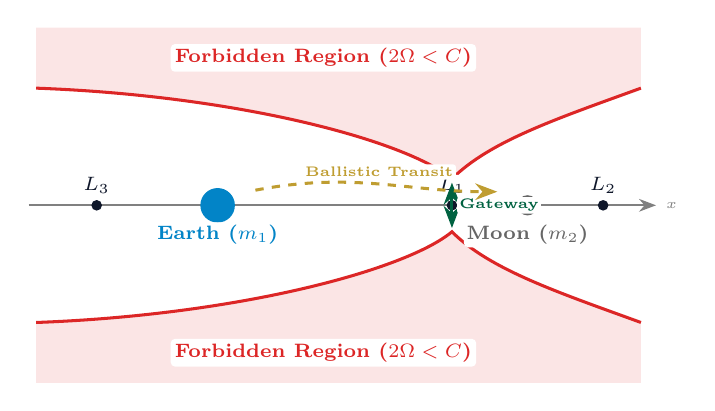
\begin{tikzpicture}[scale=0.96, >=Stealth]
                    % Synodic Centerline Axis
                    \draw[->, line width=0.7pt, Charcoal!60] (-3.9,0) -- (4.4,0) node[right, font=\tiny\bfseries] {$x$};
                    
                    % Upper Forbidden Region (Outside & Above Top Red Boundary)
                    \fill[AlertRed!12] 
                        (-3.8, 1.55) .. controls (-1.1, 1.45) and (1.1, 0.85) .. (1.7, 0.35)
                        .. controls (2.2, 0.85) and (3.1, 1.15) .. (4.2, 1.55)
                        -- (4.2, 2.35) -- (-3.8, 2.35) -- cycle;
                    \draw[line width=1.1pt, AlertRed] 
                        (-3.8, 1.55) .. controls (-1.1, 1.45) and (1.1, 0.85) .. (1.7, 0.35)
                        .. controls (2.2, 0.85) and (3.1, 1.15) .. (4.2, 1.55);
                        
                    % Upper Label: Placed clearly OUTSIDE the red line in the upper forbidden region
                    \node[font=\scriptsize\bfseries, text=AlertRed, fill=white, rounded corners=1.5pt, inner sep=1.5pt] 
                        at (0, 1.95) {Forbidden Region ($2\Omega < C$)};
                    
                    % Lower Forbidden Region (Outside & Below Bottom Red Boundary)
                    \fill[AlertRed!12] 
                        (-3.8, -1.55) .. controls (-1.1, -1.45) and (1.1, -0.85) .. (1.7, -0.35)
                        .. controls (2.2, -0.85) and (3.1, -1.15) .. (4.2, -1.55)
                        -- (4.2, -2.35) -- (-3.8, -2.35) -- cycle;
                    \draw[line width=1.1pt, AlertRed] 
                        (-3.8, -1.55) .. controls (-1.1, -1.45) and (1.1, -0.85) .. (1.7, -0.35)
                        .. controls (2.2, -0.85) and (3.1, -1.15) .. (4.2, -1.55);
                        
                    % Lower Label: Placed clearly OUTSIDE the red line in the lower forbidden region
                    \node[font=\scriptsize\bfseries, text=AlertRed, fill=white, rounded corners=1.5pt, inner sep=1.5pt] 
                        at (0, -1.95) {Forbidden Region ($2\Omega < C$)};
                    
                    % Primaries: Earth and Moon in the Allowed Corridor
                    \coordinate (E) at (-1.4, 0);
                    \coordinate (M) at (2.7, 0);
                    \fill[SpiceBlue] (E) circle (6.5pt);
                    \node[fill=white, rounded corners=1.5pt, inner sep=1pt, below=6pt, font=\scriptsize\bfseries, text=SpiceBlue] at (E) {Earth ($m_1$)};
                    \fill[gray!80!black] (M) circle (3.8pt);
                    \node[fill=white, rounded corners=1.5pt, inner sep=1pt, below=6pt, font=\scriptsize\bfseries, text=gray!80!black] at (M) {Moon ($m_2$)};
                    
                    % Lagrange Points
                    \coordinate (L1) at (1.7, 0);
                    \coordinate (L2) at (3.7, 0);
                    \coordinate (L3) at (-3.0, 0);
                    
                    \fill[DarkSlate] (L1) circle (2.0pt);
                    \node[fill=white, rounded corners=1.5pt, inner sep=1pt, above=3pt, font=\scriptsize\bfseries, text=DarkSlate] at (L1) {$L_1$};
                    \fill[DarkSlate] (L2) circle (2.0pt);
                    \node[fill=white, rounded corners=1.5pt, inner sep=1pt, above=3pt, font=\scriptsize\bfseries, text=DarkSlate] at (L2) {$L_2$};
                    \fill[DarkSlate] (L3) circle (2.0pt);
                    \node[fill=white, rounded corners=1.5pt, inner sep=1pt, above=3pt, font=\scriptsize\bfseries, text=DarkSlate] at (L3) {$L_3$};
                    
                    % Neck Opening Corridor Indicator at L1
                    \draw[<->, line width=1.1pt, UdeAGreen] (1.7, -0.30) -- (1.7, 0.30);
                    \node[right, font=\tiny\bfseries, text=UdeAGreen, fill=white, rounded corners=1pt, inner sep=0.8pt] at (1.76, 0) {Gateway};
                    
                    % Ballistic Transit Path
                    \draw[->, line width=1.1pt, dashed, UdeAGold!90!black] (-0.9, 0.20) .. controls (0.4, 0.45) and (1.1, 0.18) .. (2.3, 0.18) 
                        node[midway, above=1pt, font=\tiny\bfseries, text=UdeAGold!90!black, fill=white, inner sep=1pt, rounded corners=1pt] {Ballistic Transit};
                \end{tikzpicture}
            \end{center}
        \end{column}
        
        \begin{column}{0.42\textwidth}
            \begin{block}{\textbf{Corridor Topology vs. Energy}}
                \scriptsize
                \begin{itemize}\setlength{\itemsep}{2pt}
                    \item \textbf{Case 1 ($C > C_{L1}$):} Both primaries are enclosed in isolated potential wells. No transit is possible.
                    \item \textbf{Case 2 ($C_{L2} < C < C_{L1}$):} The $L_1$ throat opens, permitting low-energy ballistic Earth-Moon transit.
                    \item \textbf{Case 3 ($C_{L3} < C < C_{L2}$):} The $L_2$ gateway opens into interplanetary space.
                    \item \textbf{Case 4 ($C < C_{L4/L5}$):} Forbidden regions close completely; motion is unconstrained.
                \end{itemize}
            \end{block}
        \end{column}
    \end{columns}
\end{frame}

% ==============================================================================
% SLIDE 11: THE FIVE LAGRANGE POINTS
% ==============================================================================
\begin{frame}{Equilibrium Solutions: The Five Lagrange (Libration) Points}
    \begin{columns}[t]
        \begin{column}{0.50\textwidth}
            \begin{block}{\textbf{Equilibrium Condition}}
                \scriptsize
                In the synodic frame, equilibrium requires:
                \begin{equation*}
                    \dot{\mathbf{r}} = \mathbf{0} \quad \text{and} \quad \ddot{\mathbf{r}} = \mathbf{0} \implies \nabla \Omega = \mathbf{0}
                \end{equation*}
                Evaluating the out-of-plane gradient:
                \begin{equation*}
                    \frac{\partial \Omega}{\partial z} = -z\left[\frac{1-\mu}{d_1^3} + \frac{\mu}{d_2^3}\right] = 0
                \end{equation*}
                Since the bracketed term is strictly positive:
                \begin{itemize}\setlength{\itemsep}{1.5pt}
                    \item $z = 0$ identically.
                    \item \textbf{All five equilibrium points lie strictly in the primary orbital plane!}
                \end{itemize}
            \end{block}
        \end{column}
        
        \begin{column}{0.47\textwidth}
            \begin{block}{\textbf{Classification of Equilibria}}
                \scriptsize
                \begin{itemize}\setlength{\itemsep}{2.5pt}
                    \item \textbf{Collinear Points ($L_1, L_2, L_3$):}
                    Lie along the synodic $x$-axis ($y = z = 0$). Roots of Euler/Szebehely quintic polynomials. Saddle points of $\Omega$.
                    \item \textbf{Triangular Points ($L_4, L_5$):}
                    Form equilateral triangles with primaries ($d_1 = d_2 = 1$). Discovered by J.-L. Lagrange (1772):
                    \begin{equation*}
                        x = \frac{1}{2} - \mu, \quad y = \pm\frac{\sqrt{3}}{2}, \quad z = 0
                    \end{equation*}
                    Local maxima of $\Omega$ (stabilized by Coriolis gyroscopic forces if $\mu < \mu_{\text{Routh}}$).
                \end{itemize}
            \end{block}
        \end{column}
    \end{columns}
\end{frame}

% ==============================================================================
% SLIDE 12: COLLINEAR POINTS MATHEMATICS
% ==============================================================================
\begin{frame}{Solving for the Collinear Points ($L_1, L_2, L_3$)}
    \begin{columns}[t]
        \begin{column}{0.50\textwidth}
            \begin{block}{\textbf{Collinear Force Balance ($y=0, z=0$)}}
                \scriptsize
                Setting $y = 0$ in $\partial \Omega / \partial x = 0$:
                \begin{equation*}
                    x - \frac{(1-\mu)(x+\mu)}{|x+\mu|^3} - \frac{\mu(x-1+\mu)}{|x-1+\mu|^3} = 0
                \end{equation*}
                \textbf{Euler Quintic Polynomials:}
                \begin{itemize}\setlength{\itemsep}{1.5pt}
                    \item For $L_1$ ($\gamma_1 = 1 - \mu - x$):
                    {\tiny
                    \begin{equation*}
                        \gamma_1^5 - (3-\mu)\gamma_1^4 + (3-2\mu)\gamma_1^3 - \mu\gamma_1^2 + 2\mu\gamma_1 - \mu = 0
                    \end{equation*}}
                    \item For $L_2$ ($\gamma_2 = x - 1 + \mu$):
                    {\tiny
                    \begin{equation*}
                        \gamma_2^5 + (3-\mu)\gamma_2^4 + (3-2\mu)\gamma_2^3 - \mu\gamma_2^2 - 2\mu\gamma_2 - \mu = 0
                    \end{equation*}}
                \end{itemize}
            \end{block}
        \end{column}
        
        \begin{column}{0.47\textwidth}
            \begin{exampleblock}{\textbf{Earth-Moon Collinear Coordinates}}
                \scriptsize
                For Earth-Moon ($\mu \approx 0.01215$, $R \approx 384,400\text{ km}$):
                \par\vspace{2pt}
                \centering
                \resizebox{\linewidth}{!}{%
                \begin{tabular}{lcc}
                    \toprule
                    \textbf{Point} & \textbf{Synodic $x$} & \textbf{Distance to Body} \\
                    \midrule
                    $L_1$ & $+0.8369$ & $62,690\text{ km}$ (to Moon) \\
                    $L_2$ & $+1.1557$ & $64,520\text{ km}$ (to Moon) \\
                    $L_3$ & $-1.0051$ & $386,360\text{ km}$ (to Earth) \\
                    \bottomrule
                \end{tabular}%
                }
            \end{exampleblock}
            \vspace{-0.1cm}
            \begin{alertblock}{\textbf{Dynamical Instability}}
                \scriptsize
                All collinear points possess real saddle eigenvalues ($\pm \lambda$). They are dynamically unstable, enabling low-cost departure/arrival manifolds.
            \end{alertblock}
        \end{column}
    \end{columns}
\end{frame}

% ==============================================================================
% SLIDE 13: TRIANGULAR POINTS & ROUTH STABILITY
% ==============================================================================
\begin{frame}{Triangular Points ($L_4, L_5$) and The Routh Stability Criterion}
    \begin{columns}[t]
        \begin{column}{0.50\textwidth}
            \begin{block}{\textbf{Equilateral Solution ($y \neq 0$)}}
                \scriptsize
                Setting $\partial\Omega/\partial x = 0$ and $\partial\Omega/\partial y = 0$ yields:
                \begin{align*}
                    x\left[1 - \frac{1-\mu}{d_1^3} - \frac{\mu}{d_2^3}\right] - \mu(1-\mu)\left[\frac{1}{d_1^3} - \frac{1}{d_2^3}\right] &= 0 \\
                    y\left[1 - \frac{1-\mu}{d_1^3} - \frac{\mu}{d_2^3}\right] &= 0
                \end{align*}
                Since $y \neq 0$, the common term vanishes identically:
                \begin{equation*}
                    d_1 = d_2 = 1
                \end{equation*}
                $L_4$ and $L_5$ form equilateral triangles with the primaries.
            \end{block}
        \end{column}
        
        \begin{column}{0.47\textwidth}
            \begin{block}{\textbf{The Routh Stability Criterion}}
                \scriptsize
                Although potential energy is maximal at $L_4, L_5$, Coriolis forces stabilize the motion if:
                \begin{equation*}
                    \mu < \mu_{\text{Routh}} = \frac{1}{2}\left(1 - \frac{\sqrt{69}}{9}\right) \approx 0.03852
                \end{equation*}
                \textbf{Astrodynamic Context:}
                \begin{itemize}\setlength{\itemsep}{1.5pt}
                    \item \textbf{Sun-Jupiter} ($\mu \approx 9.54 \times 10^{-4}$): Trojan asteroids.
                    \item \textbf{Sun-Earth} ($\mu \approx 3.00 \times 10^{-6}$): Stable Trojan sites.
                    \item \textbf{Earth-Moon} ($\mu \approx 0.01215 < \mu_{\text{Routh}}$): Linearly stable (secularly perturbed by Sun).
                \end{itemize}
            \end{block}
        \end{column}
    \end{columns}
\end{frame}

% ==============================================================================
% SLIDE 14: LINEARIZATION AROUND COLLINEAR POINTS
% ==============================================================================
\begin{frame}{Linearization Around Collinear Libration Points}
    \begin{columns}[t]
        \begin{column}{0.49\textwidth}
            \begin{block}{\textbf{First-Order Variational Equations}}
                \scriptsize
                Let $\mathbf{x} = \mathbf{x}_{L} + \delta\mathbf{x}$ with $\delta\mathbf{x} = [\xi, \eta, \zeta, \dot{\xi}, \dot{\eta}, \dot{\zeta}]^T$:
                \begin{equation*}
                    \begin{bmatrix} \dot{\bm{\xi}} \\ \ddot{\bm{\xi}} \end{bmatrix} =
                    \begin{bmatrix}
                        \mathbf{0}_{3\times 3} & \mathbf{I}_{3\times 3} \\
                        \bm{\Omega}_{\mathbf{r}\mathbf{r}} & 2\bm{\Omega}_{\text{cor}}
                    \end{bmatrix}
                    \begin{bmatrix} \bm{\xi} \\ \dot{\bm{\xi}} \end{bmatrix}
                \end{equation*}
                where at collinear points ($y = z = 0$):
                \begin{align*}
                    \ddot{\xi} - 2\dot{\eta} &= (1 + 2\sigma)\xi \\
                    \ddot{\eta} + 2\dot{\xi} &= (1 - \sigma)\eta \\
                    \ddot{\zeta} &= -\sigma\zeta
                \end{align*}
                with $\sigma = \frac{1-\mu}{|x_L + \mu|^3} + \frac{\mu}{|x_L - 1 + \mu|^3} > 0$.
            \end{block}
        \end{column}
        
        \begin{column}{0.48\textwidth}
            \begin{block}{\textbf{Eigenstructure and Modal Dynamics}}
                \scriptsize
                The characteristic polynomial factors cleanly:
                \begin{equation*}
                    (s^2 + \sigma)\left[ s^4 + (2-\sigma)s^2 + (1+2\sigma)(1-\sigma) \right] = 0
                \end{equation*}
                \textbf{Three Decoupled Dynamical Modes:}
                \begin{itemize}\setlength{\itemsep}{2pt}
                    \item \textbf{Vertical Mode:} $s_{5,6} = \pm i\sqrt{\sigma} = \pm i\nu$ \\
                    (Pure harmonic oscillation out-of-plane).
                    \item \textbf{Saddle Mode:} $s_{1,2} = \pm \lambda$ \\
                    (Exponential unstable/stable manifolds).
                    \item \textbf{Planar Center Mode:} $s_{3,4} = \pm i\omega_p$ \\
                    (In-plane periodic Lyapunov orbits).
                \end{itemize}
            \end{block}
        \end{column}
    \end{columns}
\end{frame}

% ==============================================================================
% SLIDE 15: PERIODIC ORBIT FAMILIES
% ==============================================================================
\begin{frame}{Periodic and Quasi-Periodic Libration Orbit Families}
    \begin{columns}[t]
        \begin{column}{0.48\textwidth}
            \begin{block}{\textbf{Taxonomy of Libration Orbits}}
                \scriptsize
                \begin{itemize}\setlength{\itemsep}{3pt}
                    \item \textbf{Planar Lyapunov Orbits:} 2D periodic orbits in the $xy$-plane surrounding collinear points, oscillating between the saddle-center manifolds.
                    \item \textbf{Vertical Lyapunov Orbits:} Purely out-of-plane figure-eight periodic paths driven by the $\Omega_{zz}$ restoring frequency.
                    \item \textbf{Lissajous Orbits:} 3D quasi-periodic trajectories formed when planar ($\omega_p$) and out-of-plane ($\nu$) frequencies are incommensurate.
                    \item \textbf{Halo Orbits:} 3D periodic orbits occurring when nonlinear terms force planar and vertical frequencies to resonate ($\omega_p \approx \nu$).
                \end{itemize}
            \end{block}
        \end{column}
        
        \begin{column}{0.49\textwidth}
            \begin{block}{\textbf{Richardson's Third-Order Expansion}}
                \scriptsize
                David L. Richardson (1980) formulated an analytical perturbation solution providing initial state seeds:
                \begin{align*}
                    x(t) &= a_{21} A_x^2 + a_{22} A_z^2 - A_x \cos\tau_1 + \dots \\
                    y(t) &= k A_x \sin\tau_1 + b_{21} A_x^2 \sin 2\tau_1 + \dots \\
                    z(t) &= \pm A_z \sin\tau_1 + d_{21} A_x A_z \sin 2\tau_1 + \dots
                \end{align*}
                where $\tau_1 = \omega t + \phi$, and the amplitude constraint links $A_x$ and $A_z$:
                \begin{equation*}
                    l_1 A_x^2 + l_2 A_z^2 + \Delta = 0
                \end{equation*}
                This analytical seed serves as the input to numerical differential correctors (shooting methods).
            \end{block}
        \end{column}
    \end{columns}
\end{frame}

% ==============================================================================
% SLIDE 16: NRHO AND THE LUNAR GATEWAY
% ==============================================================================
\begin{frame}{Near-Rectilinear Halo Orbits (NRHO) and Lunar Gateway}
    \begin{columns}[t]
        \begin{column}{0.50\textwidth}
            \begin{block}{\textbf{Characteristics of NRHOs}}
                \scriptsize
                As Halo orbit amplitudes grow along the family, they become elongated near the Moon:
                \begin{itemize}\setlength{\itemsep}{1.5pt}
                    \item Near-perpendicular passage over lunar poles.
                    \item Close perilune ($1,500\text{--}3,000\text{ km}$).
                    \item High apolune ($\sim 70,000\text{ km}$) with constant line-of-sight to Earth.
                \end{itemize}
                \par\vspace{2pt}
                \textbf{Artemis Gateway 9:2 Resonant Orbit:}
                \begin{itemize}\setlength{\itemsep}{1.5pt}
                    \item Period: $\sim 6.56\text{ days}$ (9 revs per 2 synodic lunar cycles).
                    \item Completely avoids Earth eclipse shadows.
                \end{itemize}
            \end{block}
        \end{column}
        
        \begin{column}{0.47\textwidth}
            \begin{block}{\textbf{Operational Advantages for Gateway}}
                \scriptsize
                \begin{itemize}\setlength{\itemsep}{2.5pt}
                    \item \textbf{Minimal Stationkeeping:} Bounded stability requires only $\Delta V \approx 2\text{--}5\text{ m/s per year}$!
                    \item \textbf{No Communication Blackout:} Continuous line-of-sight to terrestrial ground stations.
                    \item \textbf{Efficient Staging:} Low $\Delta V$ access to Low Lunar Orbit (LLO) and the lunar South Pole.
                    \item \textbf{Flight Proven:} NASA CAPSTONE CubeSat validated this exact orbit in 2022--2023.
                \end{itemize}
            \end{block}
        \end{column}
    \end{columns}
\end{frame}

% ==============================================================================
% SLIDE 17: INVARIANT MANIFOLDS THEORY
% ==============================================================================
\begin{frame}{Invariant Manifold Theory: The Monodromy Matrix}
    \begin{columns}[t]
        \begin{column}{0.50\textwidth}
            \begin{block}{\textbf{The Monodromy Matrix ($\mathbf{M}$)}}
                \scriptsize
                For a periodic orbit $\Gamma$ of period $T$, propagate the State Transition Matrix (STM):
                \begin{equation*}
                    \dot{\bm{\Phi}}(t, t_0) = \mathbf{A}(t)\bm{\Phi}(t, t_0), \quad \bm{\Phi}(t_0, t_0) = \mathbf{I}_6
                \end{equation*}
                $\mathbf{M} = \bm{\Phi}(T, 0)$ gives the Floquet multipliers $\lambda_i$:
                \begin{itemize}\setlength{\itemsep}{1.5pt}
                    \item Symplectic symmetry enforces reciprocal pairs: $(\lambda, 1/\lambda, \bar{\lambda}, 1/\bar{\lambda})$.
                    \item Two trivial multipliers always equal unity: $\lambda_1 = \lambda_2 = 1$.
                    \item For unstable orbits: $\lambda_s < 1$ (stable) and $\lambda_u = 1/\lambda_s > 1$ (unstable).
                \end{itemize}
            \end{block}
        \end{column}
        
        \begin{column}{0.47\textwidth}
            \begin{block}{\textbf{Generating Manifold Tubes}}
                \scriptsize
                Let $\mathbf{v}_s$ and $\mathbf{v}_u$ be eigenvectors of $\mathbf{M}$ for $\lambda_s$ and $\lambda_u$:
                \begin{equation*}
                    \mathbf{x}_0^{s} = \mathbf{x}_0 \pm \epsilon \frac{\mathbf{v}_s}{\|\mathbf{v}_s\|}, \quad \mathbf{x}_0^{u} = \mathbf{x}_0 \pm \epsilon \frac{\mathbf{v}_u}{\|\mathbf{v}_u\|}
                \end{equation*}
                with perturbation $\epsilon \sim 10^{-6}\text{--}10^{-4}$.
                \begin{itemize}\setlength{\itemsep}{2pt}
                    \item \textbf{Unstable Manifold ($W^u$):} Propagate forward in time. Natural ballistic departure from orbit.
                    \item \textbf{Stable Manifold ($W^s$):} Propagate backward in time. Asymptotes onto orbit with \textbf{zero $\Delta V$}!
                \end{itemize}
            \end{block}
        \end{column}
    \end{columns}
\end{frame}

% ==============================================================================
% SLIDE 18: MANIFOLD TUBES & CISLUNAR TRANSIT (HIGH CONTRAST & VISIBLE TEXT)
% ==============================================================================
\begin{frame}{Invariant Manifold Tubes: The Interplanetary Superhighway}
    \begin{columns}[t]
        \begin{column}{0.52\textwidth}
            \begin{center}
                \vspace{-0.15cm}
                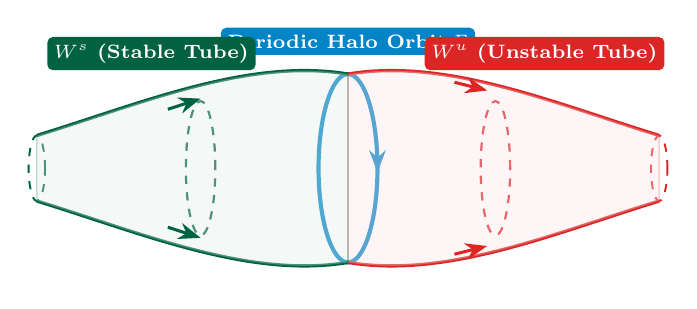
\begin{tikzpicture}[scale=1.04, >=Stealth]
                    % Periodic Halo Orbit Gamma
                    \draw[line width=1.5pt, SpiceBlue] (0,0) ellipse (0.36cm and 1.15cm);
                    \draw[->, line width=1.1pt, SpiceBlue] (0.36, 0.05) -- (0.36, -0.05);
                    
                    % Halo Orbit Label - High contrast white text on SpiceBlue badge placed clearly above
                    \node[fill=SpiceBlue, text=white, rounded corners=2pt, inner sep=2.5pt, font=\scriptsize\bfseries] 
                        at (0, 1.55) {Periodic Halo Orbit $\Gamma$};
                    
                    % Unstable Manifold Tube W^u (Flowing Rightward)
                    \draw[line width=1.2pt, AlertRed] (0, 1.15) .. controls (1.2, 1.35) and (2.5, 0.8) .. (3.8, 0.4);
                    \draw[line width=1.2pt, AlertRed] (0, -1.15) .. controls (1.2, -1.35) and (2.5, -0.8) .. (3.8, -0.4);
                    \draw[AlertRed, dashed, line width=0.8pt] (1.8, 0) ellipse (0.18cm and 0.82cm);
                    \draw[AlertRed, dashed, line width=0.7pt] (3.8, 0) ellipse (0.10cm and 0.40cm);
                    \draw[AlertRed, fill=AlertRed!12, opacity=0.35] 
                        (0, 1.15) .. controls (1.2, 1.35) and (2.5, 0.8) .. (3.8, 0.4)
                        -- (3.8, -0.4) .. controls (2.5, -0.8) and (1.2, -1.35) .. (0, -1.15) -- cycle;
                    \draw[->, line width=1.1pt, AlertRed] (1.3, 1.05) -- (1.7, 0.95);
                    \draw[->, line width=1.1pt, AlertRed] (1.3, -1.05) -- (1.7, -0.95);
                    
                    % Unstable Tube Label - High contrast white text on AlertRed badge
                    \node[fill=AlertRed, text=white, rounded corners=2pt, inner sep=2.5pt, font=\scriptsize\bfseries] 
                        at (2.4, 1.40) {$W^u$ (Unstable Tube)};
                    
                    % Stable Manifold Tube W^s (Flowing Leftward into Halo)
                    \draw[line width=1.2pt, UdeAGreen] (-3.8, 0.4) .. controls (-2.5, 0.8) and (-1.2, 1.35) .. (0, 1.15);
                    \draw[line width=1.2pt, UdeAGreen] (-3.8, -0.4) .. controls (-2.5, -0.8) and (-1.2, -1.35) .. (0, -1.15);
                    \draw[UdeAGreen, dashed, line width=0.8pt] (-1.8, 0) ellipse (0.18cm and 0.82cm);
                    \draw[UdeAGreen, dashed, line width=0.7pt] (-3.8, 0) ellipse (0.10cm and 0.40cm);
                    \draw[UdeAGreen, fill=UdeAGreen!12, opacity=0.35] 
                        (-3.8, 0.4) .. controls (-2.5, 0.8) and (-1.2, 1.35) .. (0, 1.15)
                        -- (0, -1.15) .. controls (-1.2, -1.35) and (-2.5, -0.8) .. (-3.8, -0.4) -- cycle;
                    \draw[->, line width=1.1pt, UdeAGreen] (-2.2, 0.72) -- (-1.8, 0.85);
                    \draw[->, line width=1.1pt, UdeAGreen] (-2.2, -0.72) -- (-1.8, -0.85);
                    
                    % Stable Tube Label - High contrast white text on UdeAGreen badge
                    \node[fill=UdeAGreen, text=white, rounded corners=2pt, inner sep=2.5pt, font=\scriptsize\bfseries] 
                        at (-2.4, 1.40) {$W^s$ (Stable Tube)};
                \end{tikzpicture}
            \end{center}
        \end{column}
        
        \begin{column}{0.46\textwidth}
            \begin{block}{\textbf{Cislunar Transit Architectures}}
                \scriptsize
                \begin{itemize}\setlength{\itemsep}{2pt}
                    \item \textbf{Poincaré Maps:} Manifolds intersect on surfaces of section (e.g., $y=0$), revealing transfer opportunities.
                    \item \textbf{Heteroclinic Bridges:} If $W^u(L_1)$ intersects $W^s(L_2)$, transfers between libration points require \textbf{zero $\Delta V$}!
                    \item \textbf{Ballistic Lunar Capture (GRAIL):} Passive capture via stable manifold tubes saves hundreds of m/s compared to direct insertion burns.
                \end{itemize}
            \end{block}
        \end{column}
    \end{columns}
\end{frame}

% ==============================================================================
% SLIDE 19: COMPUTATIONAL LAB 3: SYMPLECTIC VS. STANDARD INTEGRATION
% ==============================================================================
\begin{frame}{Computational Lab 3: Symplectic vs. Non-Symplectic Integrators}
    \begin{columns}[t]
        \begin{column}{0.50\textwidth}
            \begin{alertblock}{\textbf{The Failure of Standard Integrators (RK4/RK89)}}
                \scriptsize
                Runge-Kutta and Adams-Bashforth methods are designed for general ODEs:
                \begin{itemize}\setlength{\itemsep}{1.5pt}
                    \item They do \textbf{not} preserve the geometric symplectic 2-form $\omega = \sum dq_i \wedge dp_i$.
                    \item \textbf{Secular Energy Drift:} Over 100+ periods, the numerical Jacobi constant $C(t)$ exhibits irreversible systematic decay or growth.
                    \item Artificial damping or unphysical expansion alters invariant manifold boundaries.
                \end{itemize}
            \end{alertblock}
        \end{column}
        
        \begin{column}{0.47\textwidth}
            \begin{block}{\textbf{The Symplectic Sandbox Advantage}}
                \scriptsize
                Symplectic methods (Verlet, Ruth 3rd-order, Gauss-Legendre Collocation) are canonical mappings:
                \begin{itemize}\setlength{\itemsep}{1.5pt}
                    \item Preserve phase space volume exactly (Liouville's theorem).
                    \item \textbf{Bounded Energy Oscillations:} The numerical trajectory follows a perturbed "shadow Hamiltonian" $\tilde{H}$.
                    \item The Jacobi constant $C$ never drifts secularly; it remains strictly bounded for thousands of revolutions!
                \end{itemize}
            \end{block}
        \end{column}
    \end{columns}
\end{frame}

% ==============================================================================
% SLIDE 20: PYTHON IMPLEMENTATION (CR3BP ODE INTEGRATOR)
% ==============================================================================
\begin{frame}[fragile]{Python Implementation: CR3BP Equations and Jacobi Tracking}
\begin{lstlisting}[style=pythoncode]
import numpy as np
from scipy.integrate import solve_ivp

def cr3bp_derivs(t, state, mu):
    """Computes state derivatives in the CR3BP synodic rotating frame."""
    x, y, z, vx, vy, vz = state
    d1 = np.sqrt((x + mu)**2 + y**2 + z**2)
    d2 = np.sqrt((x - 1.0 + mu)**2 + y**2 + z**2)
    
    # Gravitational + Centrifugal accelerations
    ax = 2.0*vy + x - (1.0 - mu)*(x + mu)/d1**3 - mu*(x - 1.0 + mu)/d2**3
    ay = -2.0*vx + y - (1.0 - mu)*y/d1**3 - mu*y/d2**3
    az = -(1.0 - mu)*z/d1**3 - mu*z/d2**3
    return [vx, vy, vz, ax, ay, vz]

def compute_jacobi_constant(state, mu):
    """Calculates the conserved Jacobi Integral C for a given 6-state."""
    x, y, z, vx, vy, vz = state
    d1 = np.sqrt((x + mu)**2 + y**2 + z**2)
    d2 = np.sqrt((x - 1.0 + mu)**2 + y**2 + z**2)
    omega = 0.5*(x**2 + y**2) + (1.0 - mu)/d1 + mu/d2
    v_sq = vx**2 + vy**2 + vz**2
    return 2.0 * omega - v_sq

MU_EARTH_MOON = 0.0121505856
\end{lstlisting}
\end{frame}

% ==============================================================================
% SLIDE 21: MISSION DESIGN IN NASA GMAT
% ==============================================================================
\begin{frame}[fragile]{Modeling Libration Points and Rotating Frames in NASA GMAT}
    \begin{columns}[t]
        \begin{column}{0.50\textwidth}
            \begin{block}{\textbf{Transition to Operational Flight Models}}
                \scriptsize
                While CR3BP provides analytical manifold seeds, operational cislunar missions must transition into full ephemeris propagators (NASA GMAT, Copernicus):
                \begin{itemize}\setlength{\itemsep}{2pt}
                    \item In GMAT, libration points ($L_1, L_2$) are defined as dynamic celestial barycenters.
                    \item The user sets up an \texttt{ObjectReferenced} rotating frame centered on Earth-Moon $L_2$.
                \end{itemize}
            \end{block}
        \end{column}
        
        \begin{column}{0.48\textwidth}
\begin{lstlisting}[style=gmatstyle]
% Define Earth-Moon Barycenter and Libration Point
Create Barycenter EarthMoonBary;
EarthMoonBary.BodyNames = {Earth, Luna};

Create LibrationPoint EarthMoonL2;
EarthMoonL2.Primary   = Earth;
EarthMoonL2.Secondary = Luna;
EarthMoonL2.Point     = L2;

% Configure Earth-Moon Synodic Rotating Frame
Create CoordinateSystem EarthMoonRot;
EarthMoonRot.Origin    = EarthMoonL2;
EarthMoonRot.Axes      = ObjectReferenced;
EarthMoonRot.XAxis     = R;
EarthMoonRot.ZAxis     = N;
EarthMoonRot.Primary   = Earth;
EarthMoonRot.Secondary = Luna;
\end{lstlisting}
        \end{column}
    \end{columns}
\end{frame}

% ==============================================================================
% SLIDE 22: SUMMARY & NEXT STEPS
% ==============================================================================
\begin{frame}{Summary and Upcoming Computational Workshop}
    \begin{columns}[t]
        \begin{column}{0.50\textwidth}
            \begin{block}{\textbf{Key Astrodynamic Takeaways}}
                \scriptsize
                \begin{enumerate}\setlength{\itemsep}{2pt}
                    \item \textbf{The Synodic Frame:} By transforming to a frame corotating with Earth and Moon, multi-body equations become autonomous ($\dot{\mathbf{x}} = \mathbf{f}(\mathbf{x})$).
                    \item \textbf{Jacobi Invariance:} The Jacobi Constant $C$ maps Zero-Velocity Surfaces, defining physical energy corridors between primaries.
                    \item \textbf{Equilibria:} $L_1, L_2, L_3$ act as gateways; $L_4, L_5$ are gyroscopically stabilized for $\mu < 0.03852$.
                    \item \textbf{Manifolds as Trajectory Tubes:} Stable and unstable manifolds form natural, fuel-free pathways across cislunar space.
                \end{enumerate}
            \end{block}
        \end{column}
        
        \begin{column}{0.47\textwidth}
            \begin{exampleblock}{\textbf{Upcoming Tasks for Week 12}}
                \scriptsize
                \begin{itemize}\setlength{\itemsep}{2pt}
                    \item \textbf{Reading Assignment:} Battin, Ch. 8 and Koon, Lo, Marsden, Ross: \textit{Dynamical Systems, the Three-Body Problem, and Space Mission Design}.
                    \item \textbf{Computational Lab 3:}
                    Implement an implicit Gauss-Legendre integrator in Python and compare $C$-drift against standard \texttt{scipy.integrate.RK45} over 100 Halo revolutions.
                    \item \textbf{Project Milestone:} Differential correction of Southern $L_2$ Halo orbits.
                \end{itemize}
            \end{exampleblock}
        \end{column}
    \end{columns}
\end{frame}

\end{document}